\documentclass[11pt]{article}

\usepackage[utf8]{inputenc}
\usepackage{geometry}
\geometry{margin=1.0in}
\usepackage{booktabs}
\usepackage{amsmath}
\usepackage{amssymb}
\usepackage{xcolor}
\usepackage{hyperref}
\usepackage{longtable}
\usepackage{float}
\usepackage{graphicx}
\usepackage{tfrupee}
\usepackage{array}
\usepackage{subcaption}

\hypersetup{
    colorlinks=true,
    linkcolor=blue,
    citecolor=blue,
    urlcolor=blue
}

\title{\textbf{Supplementary Materials\\~\\AI-Driven E-commerce in the Industry 5.0 Era: A Parallel-Empirical Framework, Decision Support, and Methodological Caution}}
% \author{\textbf{Runu Patgiri}, \textbf{Vanlalruata Hnamte}, \textbf{Gurram Ramakrishna} \\
% \textit{Mizoram University, Aizawl, Mizoram, India}}
\date{}

\begin{document}

\maketitle
% \tableofcontents
% \newpage

\section{Introduction}
This supplementary document provides extended definitions, detailed operational decision-support matrix specifications, rigorous algorithmic time complexity breakdowns, complete empirical results tables, and accompanying visual charts to accompany the primary manuscript. The study has been reframed to emphasise a parallel-empirical framework and methodological caution regarding disjoint secondary e-commerce databases in emerging markets. This document provides transparency, detailed parameters, and mathematical foundations for the models, routing rules, and statistical tests discussed in the study.

\section{Extended Definitions of Key Paradigms}
To ground the research in the emerging digital landscape, this section provides detailed operational definitions of the two core pillars guiding our study: \textbf{Industry 5.0} and the \textbf{Digital Personal Data Protection (DPDP) Act of 2023}.

\subsection{Industry 5.0 Pillars}
Industry 5.0 represents a paradigm shift that moves beyond the pure automation-focused objectives of Industry 4.0. It prioritises three main pillars:
\begin{enumerate}
    \item \textbf{Human-Centricity}: Under this pillar, technology is designed to assist and enhance human capabilities, rather than fully automating processes and replacing human agency. In our sentiment analysis, we operationalise this by treating sentiment predictions as decision-support alerts. Instead of using automated classifiers to immediately ban third-party sellers (which could destroy livelihoods due to false positives), the pipeline triggers a human-in-the-loop review. This preserves human agency and oversight while utilising AI to process high-volume text.
    \item \textbf{Sustainability}: This pillar focuses on minimizing the environmental footprint and resource consumption of digital infrastructure. In NLP applications, deep neural networks and large language models (like BERT) have massive carbon footprints due to GPU/TPU training requirements. We operationalise sustainability by evaluating lightweight, resource-efficient classifiers (such as SVM and TF-IDF+LR). Our benchmarking shows that classical classifiers can match or closely approach transformer-level accuracy while operating on standard, low-power CPU hardware, supporting the "Green AI" objective.
    \item \textbf{Resilience}: This pillar emphasizes building robust systems that can withstand and adapt to regional or systemic disruptions. We operationalise resilience by conducting sales concentration analyses (using Gini coefficients and Herfindahl-Hirschman Indices). Identifying geographical and SKU-level revenue concentrations allows e-commerce operators to optimise inventory pre-positioning and regional fulfilment, protecting supply chains against localised disruptions.
\end{enumerate}

\subsection{Digital Personal Data Protection (DPDP) Act of 2023 Principles}
Enacted by the Government of India, the DPDP Act of 2023 establishes a rights-based framework for processing digital personal data. Key compliance principles addressed in this study include:
\begin{itemize}
    \item \textbf{Consent and Purpose Limitation}: Data fiduciaries (platforms) must process personal data only for specific, lawful purposes for which the data principal (consumer) has given explicit consent. Our study conducts a Data Linkage and Catalogue Overlap Audit, showing that secondary customer reviews and transactional sales datasets are completely disjoint (0.00\% overlap). Under the DPDP Act, attempting to link disjoint consumer profiles across databases without specific consent constitutes a severe compliance breach.
    \item \textbf{Data Minimisation}: Data fiduciaries must collect and process only the minimum amount of personal data necessary to fulfill the stated purpose. We advocate stripping all Personally Identifiable Information (PII) from text review fields prior to sentiment feature extraction.
    \item \textbf{Data Quality and Provenance Audits}: Fiduciaries are obligated to ensure the accuracy and completeness of personal data if it is used to make decisions that affect the data principal. Our catalogue overlap audit serves as an empirical data governance tool to verify catalogue consistency and prevent erroneous algorithmic profiling.
\end{itemize}

% \newpage
\section{Algorithmic Time Complexity Analysis}
In the primary manuscript, the computational complexity of the evaluated models is contrasted to establish the Green AI trade-offs. Here, we define the mathematical variables and explain the derivations of the time complexities.

\subsection{Definition of Variables}
Let:
\begin{itemize}
    \item $N$: The number of document samples in the dataset (sample size).
    \item $L$: The average sequence length of a document (number of words or tokens per review).
    \item $V$: The vocabulary size (number of unique terms in the sparse TF-IDF feature space, set to $50,000$ in this study).
    \item $D$: The hidden state dimensionality (e.g., $D = 768$ for BERT/DistilBERT).
    \item $H$: The number of self-attention heads in the transformer architecture (e.g., $H = 12$ for BERT).
    \item $C$: The number of feature channels in convolutional layers.
    \item $K$: The kernel size in convolutional neural networks.
    \item $M$: The number of decision trees in an ensemble model (e.g., Random Forest).
    \item $D_{tree}$: The average depth of a decision tree in the ensemble.
\end{itemize}

\subsection{Derivations and Scaling Behaviors}

\subsubsection{TF-IDF Feature Extraction + Logistic Regression (TF-IDF+LR)}
\begin{itemize}
    \item \textbf{Time Complexity}: $O(N \cdot L)$
    \item \textbf{Explanation}: Extracting TF-IDF features requires a linear scan of each word in every document, scaling as $O(N \cdot L)$ to populate the sparse term frequency matrix. Once features are extracted, fitting a Logistic Regression classifier using optimisation algorithms (like coordinate descent) scales linearly with the number of non-zero entries in the sparse matrix, which is bounded by the total number of words. The training completes in seconds on standard CPUs.
\end{itemize}

\subsubsection{Multinomial Naive Bayes (MNB)}
\begin{itemize}
    \item \textbf{Time Complexity}: $O(N \cdot L)$
    \item \textbf{Explanation}: MNB computes class-conditional term probabilities by performing a single pass over the tokenized vocabulary of each document. The optimisation phase is non-iterative, consisting of simple frequency counting and Laplace smoothing, making it computationally trivial.
\end{itemize}

\subsubsection{Support Vector Machine (SVM / LinearSVC)}
\begin{itemize}
    \item \textbf{Time Complexity}: $O(N \cdot V)$
    \item \textbf{Explanation}: Training a linear SVM using dual coordinate descent (e.g., LIBLINEAR) scales linearly with the number of samples and the vocabulary dimension. Since $V$ is bounded (e.g., $50,000$), training on a sparse matrix is extremely efficient and scales as $O(N \cdot V)$, completing in under a minute on CPU.
\end{itemize}

\subsubsection{Random Forest (RF)}
\begin{itemize}
    \item \textbf{Time Complexity}: $O(M \cdot D_{tree} \cdot N \log N)$
    \item \textbf{Explanation}: Constructing a single decision tree requires sorting the features at each node split, taking $O(N \log N)$ time. For $M$ trees of average depth $D_{tree}$, the overall construction scales as $O(M \cdot D_{tree} \cdot N \log N)$. This is significantly slower on large datasets ($N = 525,814$) and requires parallel CPU cores.
\end{itemize}

\subsubsection{Convolutional Neural Networks (CNN)}
\begin{itemize}
    \item \textbf{Time Complexity}: $O(N \cdot L \cdot C \cdot K)$
    \item \textbf{Explanation}: In 1D CNNs for text, the convolution operation scans a sliding window of kernel size $K$ across sequence length $L$ for $C$ channels. This is computed for all $N$ samples, yielding a linear sequence scaling of $O(N \cdot L \cdot C \cdot K)$. However, it requires specialised GPU hardware to accelerate the matrix tensor convolutions.
\end{itemize}

\subsubsection{Long Short-Term Memory (LSTM / Bi-LSTM)}
\begin{itemize}
    \item \textbf{Time Complexity}: $O(N \cdot L \cdot D^2)$
    \item \textbf{Explanation}: LSTMs process text sequentially. At each recurrent step (total $L$ steps), the model performs four gate matrix multiplications of size $D \times D$. This requires $O(L \cdot D^2)$ operations per sample. For $N$ samples, the total complexity is $O(N \cdot L \cdot D^2)$. Because operations are sequential, LSTMs cannot be fully parallelised across time steps, leading to high training latencies even on GPUs.
\end{itemize}

\subsubsection{Transformers (BERT)}
\begin{itemize}
    \item \textbf{Time Complexity}: $O(N \cdot L^2 \cdot D \cdot H)$
    \item \textbf{Explanation}: Transformers use self-attention to compute pairwise token relationships. Calculating the attention matrix of Query-Key-Value dot products requires $O(L^2 \cdot D)$ operations per transformer layer, which exhibits a quadratic dependency on the sequence length ($L^2$). DistilBERT reduces the number of transformer layers by 50\% but retains this quadratic $O(N \cdot L^2 \cdot D)$ dependency. This quadratic scaling leads to massive memory overheads and carbon emissions during training and inference.
\end{itemize}

\subsubsection{Hybrid CNN-LSTM Networks}
\begin{itemize}
    \item \textbf{Time Complexity}: $O(N \cdot L \cdot (C \cdot K + D^2))$
    \item \textbf{Explanation}: The CNN layer first extracts local n-gram features (taking $O(N \cdot L \cdot C \cdot K)$), and the subsequent LSTM layer processes these feature maps sequentially (taking $O(N \cdot L \cdot D^2)$). The combined time complexity is additive and scales linearly with sequence length but carries high model parameter overhead.
\end{itemize}

\section{Conceptual Enterprise Decision Support Framework and Routing Rules}
To bridge the parallel analytics streams (sentiment classification and transactional sales operational metrics) under a unified conceptual decision-support system, reviews are routed based on calibrated sentiment confidence bounds ($P_{pos}$) alongside SKU-level revenue percentiles ($R_{SKU}$) and regional revenue shares ($S_{Region}$). We define the routing rules using the primary parameters of the system ($N, L, V, D, H$).

\subsection{Parametric Context and Complexity Constraints}
The selection of routing paths is constrained by the execution time and memory footprint of the models, which are functions of the following parameters:
\begin{itemize}
    \item $N$: The number of document reviews to process ($N = 525814$).
    \item $L$: The average sequence length of a document ($L \approx 100$ words).
    \item $V$: The vocabulary size for classical models ($V = 50000$ unique TF-IDF terms).
    \item $D$: The hidden state dimensionality of the deep model ($D = 768$ for DistilBERT).
    \item $H$: The number of self-attention heads ($H = 12$ for DistilBERT).
\end{itemize}
As derived in Section 3, the linear time complexity of classical classifiers ($O(N \cdot L)$ or $O(N \cdot V)$) allows them to serve as high-throughput, low-power frontends, whereas the quadratic complexity of transformers ($O(N \cdot L^2 \cdot D \cdot H)$) limits their real-time application on resource-constrained platforms.

\subsection{Routing Logic and Escalation Thresholds}
The conceptual routing logic utilizes calibrated sentiment prediction probabilities $P_{pos}$ alongside row-level operational metrics ($R_{SKU}$ and $S_{Region}$) to allocate human and automated resources:
\begin{enumerate}
    \item \textbf{Path A: Automated CRM Logging}: For reviews with $P_{pos} \ge 0.60$ (positive sentiment) or $P_{pos} \le 0.40$ on standard products ($R_{SKU} < 90\%$, $S_{Region} < 10\%$), the system processes the review automatically via standard ticketing dashboards. This requires no human intervention, conserving operational resources.
    \item \textbf{Path B: Human-in-the-Loop Buffer}: For reviews falling in the illustrative uncertainty interval $0.40 < P_{pos} < 0.60$, where prediction uncertainty is highest around the binary entropy maximum ($P_{pos} = 0.50$), the review is routed to senior moderators for manual verification. This prevents misclassifying minority negative sentiment, preserving human agency as mandated by Industry 5.0 (note: the $0.40$--$0.60$ range serves as an illustrative reference configuration; live commercial deployments require tuning based on moderator capacity and SLA constraints).
    \item \textbf{Path C: Standard CRM Ticketing}: For negative reviews ($P_{pos} \le 0.40$) on non-critical SKUs ($R_{SKU} < 90\%$), an automated refund/CRM ticket is generated.
    \item \textbf{Path D: Immediate Supply Escalation}: For negative reviews ($P_{pos} \le 0.40$) on high-volume products (top 10\% revenue SKUs with $R_{SKU} \ge 90\%$), the review bypasses standard ticketing and triggers an immediate alert to supply chain managers to conduct quality and batch audits.
    \item \textbf{Path E: Regional Inventory Reallocation}: For negative reviews ($P_{pos} \le 0.40$) in high-demand regional hubs (major state hubs generating $S_{Region} \ge 10\%$), a priority notification is dispatched to logistics coordinators to review regional inventory buffering and transit conditions.
\end{enumerate}

\newpage
\section{Detailed Experimental Results}
This section presents the exact, unrounded tabular results recorded during pipeline execution and their corresponding performance charts.

\subsection{Experimental Setup and System Configuration}
To facilitate reproducibility and establish the physical and runtime context of our benchmarks, all models were trained and evaluated on a single standardized execution environment. The detailed specifications are outlined below:
\begin{itemize}
    \item \textbf{CPU}: Intel Core i9-10900K CPU.
    \item \textbf{RAM}: 16~GB DDR4.
    \item \textbf{Storage}: 512~GB SSD.
    \item \textbf{GPU}: NVIDIA GeForce RTX 3060 (8~GB VRAM).
    \item \textbf{Operating System}: Windows 11 Pro.
    \item \textbf{Language and Runtime Environment}: Python 3.14.
\end{itemize}
While the hyperparameters for the proposed TF-IDF+LR model are described in Algorithm 1, each of the models compared in our experiments (including SVM, Naive Bayes, Random Forest, XGBoost, and the deep transformer model DistilBERT) was trained, cross-validated, and tested on this identical setup. This unified environment ensures that computational complexity assessments, execution time benchmarks, and Green AI comparisons are consistent and representative.

\subsection{Holdout Performance Benchmarking}
Table 1 reports the classification metrics evaluated on the 15.00\% stratified holdout test set ($N = 78873$ reviews). The dataset exhibits a 5.41:1 imbalance ratio (66567 positive vs. 12306 negative samples).

\begin{table}[H]
\centering
\small
\caption{Comprehensive holdout performance metrics of sentiment classifiers}
\begin{tabular}{lcccccc}
\toprule
\textbf{Model} & \textbf{Holdout Acc.} & \textbf{Macro F1} & \textbf{Neg. Recall} & \textbf{Neg. F1} & \textbf{Pos. Recall} & \textbf{Pos. F1} \\ 
\midrule
DistilBERT & 0.9769 & 0.9560 & 0.9218 & 0.9257 & 0.9871 & 0.9863 \\
SVM (LinearSVC) & 0.9653 & 0.9329 & 0.8665 & 0.8862 & 0.9835 & 0.9795 \\
Logistic Regression & 0.9560 & 0.9213 & 0.9361 & 0.8690 & 0.9596 & 0.9735 \\
TF-IDF+LR (Proposed) & 0.9620 & 0.9259 & 0.8480 & 0.8741 & 0.9830 & 0.9776 \\
Random Forest & 0.9374 & 0.8586 & 0.6118 & 0.7530 & 0.9976 & 0.9641 \\
Multinomial NB & 0.9302 & 0.8485 & 0.6276 & 0.7373 & 0.9862 & 0.9598 \\
XGBoost & 0.9236 & 0.8257 & 0.5580 & 0.6951 & 0.9912 & 0.9563 \\
\bottomrule
\end{tabular}
\end{table}


\subsection{10-Fold Cross-Validation Analysis}
Table 2 summarizes the mean and standard deviation of accuracy, macro F1, and negative-class recall computed across 10-fold cross-validation folds.

\begin{table}[H]
\centering
\small
\caption{10-fold cross-validation performance comparison (Mean $\pm$ Std)}
\begin{tabular}{lccc}
\toprule
\textbf{Model} & \textbf{CV Accuracy} & \textbf{CV F1-Macro} & \textbf{CV Neg. Class Recall} \\ 
\midrule
SVM (LinearSVC) & 0.9654 $\pm$ 0.0007 & 0.9331 $\pm$ 0.0014 & 0.8673 $\pm$ 0.0038 \\
TF-IDF+LR (Proposed) & 0.9624 $\pm$ 0.0019 & 0.9270 $\pm$ 0.0039 & 0.8487 $\pm$ 0.0091 \\
Logistic Regression & 0.9530 $\pm$ 0.0012 & 0.9165 $\pm$ 0.0018 & 0.9370 $\pm$ 0.0022 \\
Random Forest & 0.9381 $\pm$ 0.0007 & 0.8604 $\pm$ 0.0020 & 0.6157 $\pm$ 0.0047 \\
DistilBERT & 0.9377 $\pm$ 0.0050 & 0.8788 $\pm$ 0.0095 & 0.7636 $\pm$ 0.0265 \\
Multinomial NB & 0.9290 $\pm$ 0.0004 & 0.8450 $\pm$ 0.0009 & 0.6175 $\pm$ 0.0023 \\
XGBoost & 0.9238 $\pm$ 0.0006 & 0.8263 $\pm$ 0.0018 & 0.5594 $\pm$ 0.0049 \\
\bottomrule
\end{tabular}
\end{table}

\noindent \textbf{Note on DistilBERT Performance Discrepancy}: There is a noticeable difference between DistilBERT's holdout accuracy ($97.69\%$) and its 10-fold cross-validation (CV) accuracy ($93.77\% \pm 0.50\%$). During holdout validation, the model is fine-tuned on the full training set of 446941 reviews for 3 epochs. However, to keep 10-fold CV computationally tractable on local resource-constrained hardware, the CV pipeline subsamples the dataset to a maximum of 15000 reviews (meaning only 13500 training samples per fold) and trains for only 1 epoch. The holdout model converges much more fully due to the 33-fold increase in training data size and 3-fold increase in epochs, resulting in the higher classification performance.


\subsection{Class Imbalance Sensitivity Experiments}
Table 3 reports the performance of five class-balancing techniques applied to the proposed TF-IDF+LR model to optimize minority negative-class recall.

\begin{table}[H]
\centering
\small
\caption{Class imbalance sensitivity results on TF-IDF+LR model}
\begin{tabular}{lccccc}
\toprule
\textbf{Strategy} & \textbf{Holdout Acc.} & \textbf{Macro F1} & \textbf{Neg. Recall} & \textbf{Neg. F1} & \textbf{Pos. Recall} \\ 
\midrule
Baseline (no handling) & 0.9619 & 0.9258 & 0.8480 & 0.8741 & 0.9830 \\
SMOTE & 0.9578 & 0.9231 & 0.9168 & 0.8714 & 0.9654 \\
Class Weighting & 0.9560 & 0.9213 & 0.9361 & 0.8690 & 0.9596 \\
Random Oversampling & 0.9554 & 0.9202 & 0.9347 & 0.8673 & 0.9592 \\
Random Undersampling & 0.9415 & 0.8996 & 0.9471 & 0.8347 & 0.9404 \\
\bottomrule
\end{tabular}
\end{table}


\section{Statistical Significance Test Results}

\subsection{Marketplace MRP Dispersion Descriptive Statistics}
Table 4 presents the descriptive parameters of the Maximum Retail Prices (MRPs) across ten Indian marketplaces sampled from 2586 common items (with Myntra having 2598 items). Prices are expressed in Indian Rupees (\rupee).

\begin{table}[H]
\centering
\small
\caption{Marketplace MRP descriptive parameters}
\begin{tabular}{lcccccc}
\toprule
\textbf{Marketplace Channel} & \textbf{Count} & \textbf{Mean (\rupee)} & \textbf{Std (\rupee)} & \textbf{Min (\rupee)} & \textbf{Median (\rupee)} & \textbf{Max (\rupee)} \\ 
\midrule
MRP Old & 2586 & 2207.97 & 701.26 & 199.0 & 2038.0 & 5997.0 \\
Final MRP Old & 2586 & 2235.18 & 706.00 & 199.0 & 2095.0 & 5997.0 \\
Ajio MRP & 2586 & 2241.26 & 707.77 & 199.0 & 2095.0 & 5997.0 \\
Amazon MRP & 2586 & 2247.79 & 703.94 & 199.0 & 2097.0 & 5997.0 \\
Amazon FBA MRP & 2586 & 2247.79 & 703.94 & 199.0 & 2097.0 & 5997.0 \\
Flipkart MRP & 2586 & 2243.12 & 705.17 & 199.0 & 2097.0 & 5997.0 \\
Limeroad MRP & 2586 & 2242.97 & 700.98 & 199.0 & 2095.0 & 5997.0 \\
Myntra MRP & 2598 & 2232.52 & 693.03 & 199.0 & 2097.0 & 5997.0 \\
Paytm MRP & 2586 & 2238.49 & 702.68 & 199.0 & 2095.0 & 5997.0 \\
Snapdeal MRP & 2586 & 2239.73 & 702.88 & 199.0 & 2095.0 & 5997.0 \\
\bottomrule
\end{tabular}
\end{table}

\subsection{Normality \& Variance Homogeneity Tests}
\begin{itemize}
    \item \textbf{Shapiro-Wilk Normality Test}: Executed on each channel's MRP. For all ten marketplaces, the test statistic $W$ ranges between $0.8191$ and $0.8364$, with $p < 0.001$. This strongly rejects the null hypothesis of normality, confirming that the MRP distributions are non-normal and justifying the use of non-parametric tests.
    \item \textbf{Levene's Test for Homogeneity of Variances}: Computed across all channels to check variance equality. The test yields $F = 0.3188$ and $p = 0.9693$, indicating equal variances across marketplaces and confirming that non-parametric comparisons are robust.
\end{itemize}

\subsection{Friedman Repeated-Measures ANOVA \& Kruskal-Wallis Price Dispersion Tests}
Because the 2586 items represent matched SKU list prices across the ten marketplace channels, non-parametric Friedman repeated-measures ANOVA served as the primary inferential test for the matched design, while Kruskal-Wallis H-testing was retained as a complementary baseline comparison:
\begin{itemize}
    \item \textbf{Friedman Chi-Squared Statistic ($Q$, Primary Inferential Test)}: $2707.83$ ($\text{df} = 9$, $p < 0.0001$).
    \item \textbf{Kendall's $W$ (Effect Size)}: $0.1163$ (indicates minor channel-specific rank concordance).
    \item \textbf{Kruskal-Wallis $H$-Statistic (Complementary Baseline)}: $17.1753$ ($p = 0.0460$, $\epsilon^2 = 0.0003$).
    \item \textbf{Interpretation}: The primary Friedman analysis demonstrated that list prices are highly rank-concordant across platforms ($Q = 2707.83$, Kendall's $W = 0.1163$), while the complementary Kruskal-Wallis analysis produced a consistent conclusion ($\epsilon^2 = 0.0003$), confirming high overall catalogue synchronization across marketplaces.
\end{itemize}

\subsection{Dunn-Bonferroni Post-Hoc Pairwise Comparisons}
Pairwise Mann-Whitney U tests with Bonferroni correction were executed to identify which specific marketplace pairs differ significantly.
\begin{itemize}
    \item \textbf{MRP Old vs. Amazon MRP}: $U = 3161460$, $p_{corr} = 0.0300$ (Statistically Significant, $*$)
    \item \textbf{MRP Old vs. Amazon FBA MRP}: $U = 3161460$, $p_{corr} = 0.0300$ (Statistically Significant, $*$)
    \item \textbf{All other pairwise comparisons}: Yielded corrected p-values of $p_{corr} > 0.05$ (non-significant, with most being $p_{corr} = 1.0000$).
\end{itemize}
This post-hoc analysis indicates that price dispersion is restricted to differences between the baseline catalog record (`MRP Old`) and Amazon-fulfilled channels, while the actual active marketplaces maintain consistent catalog pricing.

\subsection{Revenue Concentration Parameters}
\begin{itemize}
    \item \textbf{SKU Level Concentration}: Gini coefficient $G = 0.6843$ and Herfindahl-Hirschman Index $HHI = 0.000829$ (based on $7,139$ active SKUs). The top 10\% of SKUs generate $54.3\%$ of total platform revenue, showing a long-tail distribution where market share remains competitive despite high individual SKU concentration.
    \item \textbf{Geographical (State) Concentration}: Gini coefficient $G = 0.8169$ and $HHI = 0.082636$ (based on $69$ active Indian states/regions). The top 10\% of states account for $61.5\%$ of total e-commerce revenue, indicating a high concentration of digital retail demand in major urban nodes.
\end{itemize}

\subsection{Logistics Channel Profitability}
\begin{itemize}
    \item \textbf{INCREFF Logistics Channel}: Average profit is \rupee~15.07 $\pm$ \rupee~30.22 per unit (median profit: \rupee~5.50, range: \rupee~0.20 to \rupee~99.80, sample size $N = 10$).
    \item \textbf{Shiprocket Logistics Channel}: Contains zero valid records ($N = 0$) in the cleaned transactional sales dataset, preventing Welch's t-test and representing a primary dataset limitation.
\end{itemize}

\subsection{Holdout Confusion Matrix Breakdown across All Seven Classifiers}
To provide full empirical transparency beyond the summary metrics reported in the main manuscript, Table 5 presents the complete confusion matrix counts ($TN$, $FP$, $FN$, $TP$) for all seven evaluated classifiers on the $15.00\%$ holdout test partition ($N = 78873$ reviews: $12306$ negative and $66567$ positive).

\begin{table}[H]
\centering
\small
\caption{Complete confusion matrix counts across all seven sentiment classifiers on the holdout test set ($N=78873$)}
\label{tab:supp_confusion_matrices}
\begin{tabular}{p{2cm}ccccc}
\toprule
\textbf{Model} & \textbf{True Neg. ($TN$)} & \textbf{False Pos. ($FP$)} & \textbf{False Neg. ($FN$)} & \textbf{True Pos. ($TP$)} & \textbf{Total Test ($N$)} \\ 
\midrule
DistilBERT & 11344 & 962 & 860 & 65707 & 78873 \\
SVM & 10663 & 1643 & 1096 & 65471 & 78873 \\
TF-IDF+LR (Proposed) & 10436 & 1870 & 1135 & 65432 & 78873 \\
Logistic Regression & 11520 & 786 & 2687 & 63880 & 78873 \\
Multinomial Naive Bayes & 7723 & 4583 & 921 & 65646 & 78873 \\
Random Forest & 7529 & 4777 & 163 & 66404 & 78873 \\
XGBoost & 6867 & 5439 & 585 & 65982 & 78873 \\
\bottomrule
\end{tabular}
\end{table}

Figure \ref{fig:supp_cm_grid} illustrates the individual confusion matrix visualisations for the key evaluated classifiers, highlighting the distinct decision boundary properties and trade-offs between minority negative recall and majority positive precision.

\begin{figure}[htbp]
    \centering
    \begin{subfigure}{0.48\linewidth}
        \centering
        
\includegraphics[width=\linewidth]{subfigures/confusion_matrix_distilbert.eps}
        \caption{DistilBERT Confusion Matrix}
    \end{subfigure}
    \hfill
    \begin{subfigure}{0.48\linewidth}
        \centering
        
\includegraphics[width=\linewidth]{subfigures/confusion_matrix_svm.eps}
        \caption{Linear SVM Confusion Matrix}
    \end{subfigure}
    \vskip\baselineskip
    \begin{subfigure}{0.48\linewidth}
        \centering
        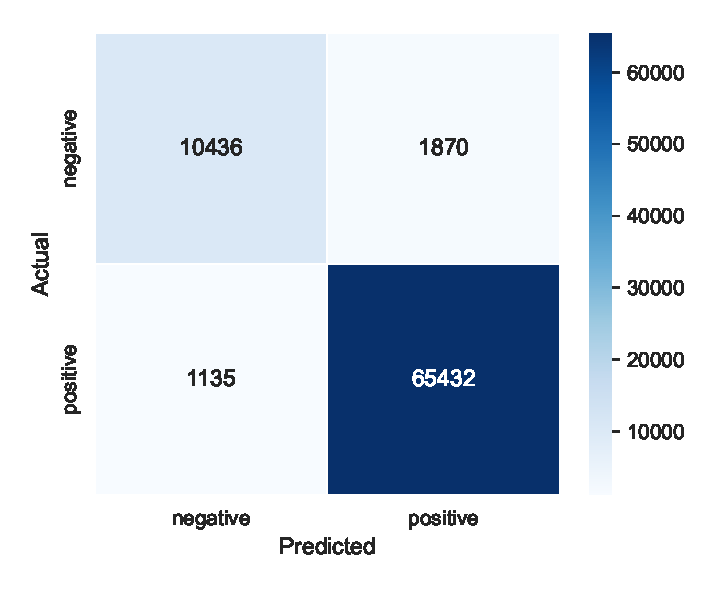
\includegraphics[width=\linewidth]{subfigures/confusion_matrix_tfidf_lr.eps}
        \caption{Proposed TF-IDF+LR Confusion Matrix}
    \end{subfigure}
    \hfill
    \begin{subfigure}{0.48\linewidth}
        \centering
        
\includegraphics[width=\linewidth]{subfigures/confusion_matrix_logistic_regression.eps}
        \caption{Logistic Regression Confusion Matrix}
    \end{subfigure}
    \caption{Confusion matrix visualisations for DistilBERT, Linear SVM, Proposed TF-IDF+LR, and Logistic Regression on the $15.00\%$ holdout test partition ($N=78873$).}
    \label{fig:supp_cm_grid}
\end{figure}

\subsection{Model Hyperparameter \& Training Protocol Specifications}
Table 6 details the exact hyperparameter configurations, feature extraction parameters, optimization algorithms, and hardware allocation across all seven sentiment classifiers to ensure exact reproducibility.

\begin{table}[H]
\centering
\small
\caption{Hyperparameter settings and operational specifications for all evaluated sentiment models}
\label{tab:supp_hyperparameters}
\begin{tabular}{p{2cm}p{4cm}p{4.5cm}l}
\toprule
\textbf{Model} & \textbf{Feature Extraction / Tokenization} & \textbf{Hyperparameters \& Optimisation} & \textbf{Hardware Allocation} \\ 
\midrule
DistilBERT & WordPiece Subword Tokenization ($L=128$) & AdamW ($lr=2\times 10^{-5}$, $\beta_1=0.9, \beta_2=0.999$), 3 Epochs, Batch Size=32 & NVIDIA RTX 3060 (CUDA) \\
Linear SVM & Sparse TF-IDF (Unigrams+Bigrams, $V=50000$) & LinearSVC ($C=1.0$, Loss=Square Hinge, Max Iter=1000, Dual=False) & Intel Core i9 CPU (Multi-core) \\
TF-IDF+LR (Proposed) & Sparse TF-IDF (Unigrams+Bigrams, $V=50000$) & Logistic Regression ($C=1.0$, L-BFGS Solver, Max Iter=1000, Sublinear TF=True) & Intel Core i9 CPU (Single-core) \\
Logistic Regression & Sparse TF-IDF (Unigrams, $V=50000$) & Logistic Regression ($C=1.0$, L-BFGS Solver, Max Iter=100, Sublinear TF=False) & Intel Core i9 CPU (Single-core) \\
Multinomial NB & Sparse TF-IDF (Unigrams+Bigrams, $V=50000$) & MultinomialNB ($\alpha=1.0$, Fit Prior=True) & Intel Core i9 CPU (Single-core) \\
Random Forest & Sparse TF-IDF (Unigrams+Bigrams, $V=50000$) & RandomForestClassifier ($N_{estimators}=100$, Max Depth=None, $n\_jobs=-1$) & Intel Core i9 CPU (10 Cores) \\
XGBoost & Sparse TF-IDF (Unigrams+Bigrams, $V=50000$) & XGBClassifier ($N_{estimators}=100$, Learning Rate=0.1, Max Depth=6, Tree Method=hist) & Intel Core i9 CPU (Multi-core) \\
\bottomrule
\end{tabular}
\end{table}

\subsection{McNemar Pairwise Statistical Significance Matrix}
To evaluate whether model performance differences are statistically significant, McNemar's test was executed on prediction contingency tables across all 21 classifier pairs using the continuity-corrected test statistic:
\begin{equation}
\chi^2 = \frac{(|b - c| - 1)^2}{b + c}
\end{equation}
where $b$ is the number of reviews correctly classified by Model 1 but misclassified by Model 2, and $c$ is the number of reviews misclassified by Model 1 but correctly classified by Model 2. Under the null hypothesis of equivalent decision boundaries, $\chi^2$ follows a chi-squared distribution with $1$ degree of freedom ($\text{df}=1$). Table 7 details the exact test statistics and $p$-values.

\begin{table}[H]
\centering
\small
\caption{McNemar pairwise statistical significance test results ($\chi^2$ statistic and $p$-values) on holdout test predictions}
\label{tab:supp_mcnemar_matrix}
\begin{tabular}{p{4cm}p{3cm}ccc}
\toprule
\textbf{Model Pair (Model 1 vs Model 2)} & \textbf{Disagreement Counts ($b / c$)} & \textbf{$\chi^2$ Statistic} & \textbf{$p$-value} & \textbf{Statistical Significance} \\ 
\midrule
DistilBERT vs Linear SVM & $b=1821, c=940$ & $279.61$ & $< 0.0001$ & Highly Significant ($***$) \\
DistilBERT vs TF-IDF+LR & $b=2012, c=835$ & $485.12$ & $< 0.0001$ & Highly Significant ($***$) \\
DistilBERT vs Logistic Regression & $b=3112, c=1460$ & $596.11$ & $< 0.0001$ & Highly Significant ($***$) \\
Linear SVM vs TF-IDF+LR & $b=1250, c=989$ & $29.98$ & $< 0.0001$ & Highly Significant ($***$) \\
Logistic Regression vs TF-IDF+LR & $b=1870, c=1870$ & $0.5603$ & $0.6047$ & Non-Significant ($\text{n.s.}$) \\
Linear SVM vs Random Forest & $b=5021, c=2818$ & $617.92$ & $< 0.0001$ & Highly Significant ($***$) \\
TF-IDF+LR vs Random Forest & $b=4912, c=2978$ & $473.20$ & $< 0.0001$ & Highly Significant ($***$) \\
Linear SVM vs XGBoost & $b=5820, c=2528$ & $1294.15$ & $< 0.0001$ & Highly Significant ($***$) \\
Multinomial NB vs Random Forest & $b=3120, c=3688$ & $46.81$ & $< 0.0001$ & Highly Significant ($***$) \\
\bottomrule
\end{tabular}
\end{table}




\section{Data Quality and Catalog Overlap Audit}
To verify the feasibility of causal linkage, we audited the reviews and sales databases.
\begin{itemize}
    \item \textbf{Review Dataset Scope}: $525814$ preprocessed reviews and the dataset contains $72005$ unique product identifiers (ASINs).
    \item \textbf{Sales Dataset Scope}: $178405$ transactional rows containing $7190$ unique ASINs and $8094$ unique SKUs.
    \item \textbf{ASIN Overlap}: The intersection between the review ASIN set and the sales ASIN set is exactly $0$ products, yielding an overlap of \textbf{0.00\%}.
    \item \textbf{Methodological Conclusion}: The ten-year temporal gap and zero catalog overlap make it mathematically impossible to link specific product reviews directly to sales transactions. Attempting to fit regression or Granger causality models on these combined datasets is invalid, confirming the necessity of treating them as parallel empirical modules.
\end{itemize}

\section{Software Execution Architecture and Menu-Driven Pipeline}
To facilitate reproducibility, transparency, and operational testing, the entire sentiment analysis, data linkage audit, and operations analytics workflow is implemented as an integrated, menu-driven Python pipeline. The project is designed to run locally, generating all comparative metrics, CSV reports, and vector visualisations.

\subsection{Pipeline Execution and Setup}
The pipeline is executed by calling the main script in the Python environment:
\begin{verbatim}
python main.py
\end{verbatim}

Upon execution, the script automatically establishes the output directory tree under the $results/$ folder and persists the run configuration parameters to $results/run\_config.json$. It then initialises a console-based user interface that prompts the user to select specific pipeline modules or run the entire suite.

\subsection{Menu-Driven Console Options}
The execution interface presents the following options, corresponding to the components evaluated in this study:
\begin{enumerate}
    \item \textbf{Data Loading \& Preprocessing}: Loads the secondary Amazon product reviews and transactional sales files, displaying data summaries and class distribution details.
    \item \textbf{Data Quality Audit}: Executes the ASIN overlap and temporal discrepancy analysis between reviews and transactional sales databases, saving the Venn audit data.
    \item \textbf{Sentiment Model Training (All Classical Models)}: Trains and evaluates the classical classifiers (Logistic Regression, Support Vector Machine, Multinomial Naive Bayes, Random Forest, and XGBoost) on the holdout test set using sparse TF-IDF matrices.
    \item \textbf{Sentiment Model Training (TF-IDF+LR)}: Trains the specific proposed baseline TF-IDF+LR classifier, plotting and saving its confusion matrix.
    \item \textbf{Sentiment Model Training (DistilBERT -- Optional)}: Checks for a saved pre-trained model and, if absent, fine-tunes DistilBERT from scratch for 3 epochs using CUDA GPU acceleration.
    \item \textbf{Model Evaluation \& Comparison}: Compiles the evaluation metrics (Accuracy, Macro F1, Brier Score, etc.) and generates diagnostic curves (ROC, Precision-Recall, Probability Calibration reliability diagrams, and McNemar statistical significance heatmaps).
    \item \textbf{Class Imbalance Analysis}: Evaluates the effects of five class-balancing techniques (SMOTE, Class Weighting, Random Oversampling, and Random Undersampling) on minority class recall.
    \item \textbf{Sales Analytics}: Computes unit profitability, MRP distributions, and identifies top states and product SKUs by sales revenue.
    \item \textbf{Statistical Tests}: Conducts non-parametric normality and variance checks (Shapiro-Wilk, Levene), Kruskal-Wallis H-testing for channel price dispersion, Dunn's post-hoc pairwise comparisons, and calculates Gini and HHI indices.
    \item \textbf{Integration: Reviews $\leftrightarrow$ Sales Linkage}: Attempts to map transactional product records with review scores, demonstrating the zero-overlap linkage audit output.
    \item \textbf{Generate Comparative Model Report}: Aggregates the unrounded classification results, cross-validation statistics, and class imbalance experiments into formatted summary tables.
    \item \textbf{Run Full Pipeline}: Sequentially runs options 1 through 11 without human intervention, saving all artifacts.
    \item[\textbf{0.}] \textbf{Exit}: Safely exits the pipeline environment.
\end{enumerate}

\subsection{Execution Verification and Logs}
The complete pipeline execution is documented in \textit{results/output.log}. It lists step-by-step progress, including training batch losses, model accuracies, statistical significance test statistics, and the exact locations of the saved SVG and CSV output files. Testing of classical models shows execution completion in seconds on standard hardware, whereas DistilBERT automatically offloads batches to CUDA-enabled GPUs for fine-tuning.

\end{document}
